\documentclass[]{article}
\usepackage[round]{natbib}

\usepackage{fullpage}
\usepackage{url}
\usepackage{authblk}
\usepackage{graphicx}
\usepackage{color}
\usepackage{booktabs}
\usepackage{bm}

% cross-reference with main text
\usepackage{xr}
\externaldocument{manuscript}

% local definitions
\newcommand{\aprcomment}[1]{{\textcolor{blue}{Comment: #1}}}

\usepackage{xspace}
\newcommand{\moments}{\texttt{moments}\xspace}
\newcommand{\fwdpy}{\texttt{fwdpy11}\xspace}

\title{Supporting Information for\\
``Archaic introgression and the distribution
of shared variation under stabilizing selection''}
\author[]{Aaron P. Ragsdale}
\affil[]{Department of Integrative Biology, University of Wisconsin--Madison, WI, USA}
\date{\today}

\begin{document}
\maketitle

\renewcommand{\thesection}{S\arabic{section}}
\renewcommand{\thetable}{S\arabic{table}}
\renewcommand{\thefigure}{S\arabic{figure}}

\section{Supplemental Figures}

\begin{figure}[ht!]
    \centering
    \includegraphics{../figures/one_pop_supp.pdf}
    \caption{
        Single-population dynamics when $V_G$ is not small.
        Solid lines: expected $V_G$ assuming $s=a^2/2V_S$. Dashed lines:
        expected $V_G$ assuming $s=a^2/2(V_S+V_G)$. When mutation rates
        are large (here, $\mu=0.01$, $V_S=1$), $V_G$ is non-negligible
        compared to $V_S$. By having to account for $V_G$ in the
        translation of effect size to selection coefficient, it makes
        $s$ non-constant if $V_G$ changes over time (due to non-constant
        demography, for example). In this case, $s$ must be updated
        regularly, given the current state of the population.
        Here, the demographic history is a bottleneck followed by a
        recovery, as depicted in Figure~\ref{fig:one-pop}A.
    }
    \label{fig:supp-one-pop}
\end{figure}

\begin{figure}[ht!]
    \centering
    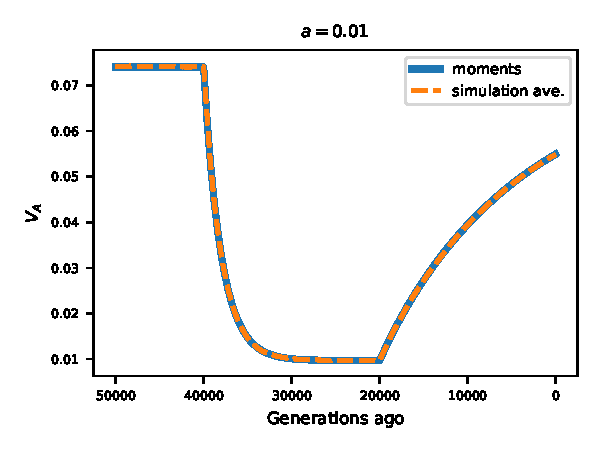
\includegraphics{../figures/one_pop.a_0.01.pdf}
    \caption{
        Simulations with no linkage and weak effects.
        Total mutation rate was $\mu=0.025$ and all mutations had effect
        sizes $a=\pm 0.01$. The demographic history (bottleneck and
        recovery) is depicted in Figure~\ref{fig:one-pop}A. The predicted
        trajectory of additive genetic variance using \moments was found
        assuming symmetric underdominant selection on trait-affecting
        alleles, with selection coefficient $s=a^2/2(V_S+V_G)$.
    }
    \label{fig:one-pop-0.01}
\end{figure}

\begin{figure}[ht!]
    \centering
    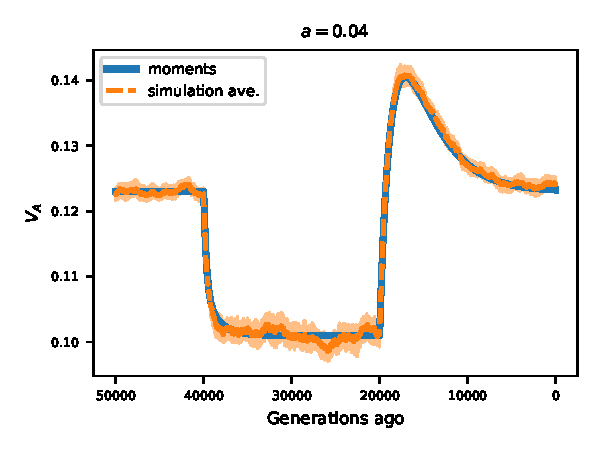
\includegraphics{../figures/one_pop.a_0.04.pdf}
    \caption{
        Simulations with no linkage and moderate effects.
        All parameters were consistent with Figure~\ref{fig:one-pop-0.01},
        but with effect sizes $a=\pm0.04$.
    }
    \label{fig:one-pop-0.04}
\end{figure}

\begin{figure}[ht!]
    \centering
    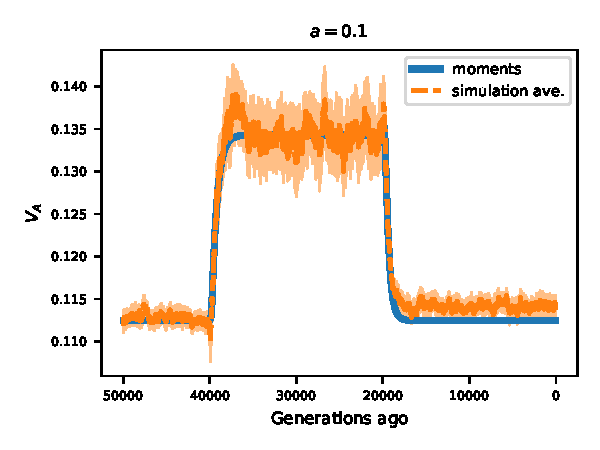
\includegraphics{../figures/one_pop.a_0.1.pdf}
    \caption{
        Simulations with no linkage and strong effects.
        All parameters were consistent with Figure~\ref{fig:one-pop-0.01}, 
        but with effect sizes $a=\pm0.1$. In each comparison (weak, moderate,
        and strong effect sizes), predictions from \moments closely match
        observed average additive genetic variance from simulations.
    }
    \label{fig:one-pop-0.1}
\end{figure}


\begin{figure}[ht!]
    \centering
    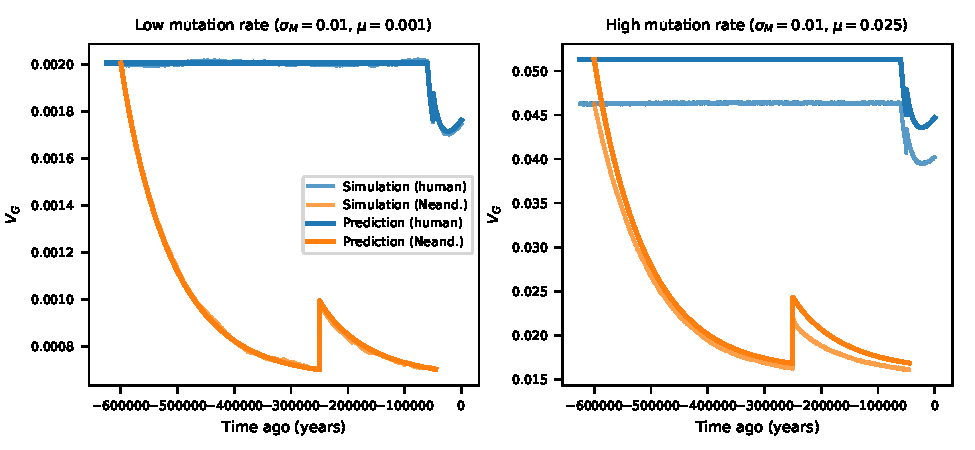
\includegraphics{../figures/model_comparison.SD_0.01.mu_0.001_0.025.pdf}
    \caption{
        With low mutational variance ($V_M=0.0001$), individual-based simulations
        using \fwdpy closely match our predictions using \moments, when the
        mutation rate is small (Left). When the mutation rate is increased,
        polygenicity increases and unlinked expectations from \moments deviate
        from observed $V_G$ in individual-based simulations. In this case, with
        relatively small mutational variance, the observed $V_G$ is reduced in
        comparison, consistent with the Bulmber (1971) effect.
    }
    \label{fig:supp-low-VM}
\end{figure}

\begin{figure}[ht!]
    \centering 
    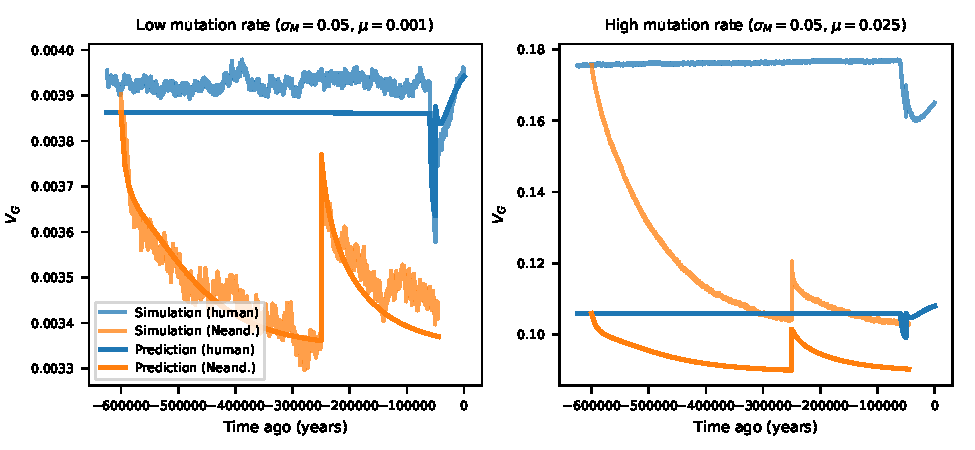
\includegraphics{../figures/model_comparison.SD_0.05.mu_0.001_0.025.pdf}
    \caption{
        With high mutational variance ($V_M=0.0025$), strong deviations are
        observed between individual-based simulations and expectations without
        linkage. When the mutational input is large, observed $V_G$ can be
        much larger than expectations without linkage, possibly consistent with
        widespread interference between alleles.
    }
    \label{fig:supp-high-VM}
\end{figure}

\begin{figure}[t!]
    \centering
    \includegraphics{../figures/human-neand-VG.pdf}
    \caption{
        Genetic variance of a trait under stabilizing selection in a model with
        human (blue) and Neanderthal (orange) demography. We consider two
        mutational variances ($\sigma_M=0.05$ and $0.01$). The demographic model
        (Figure~\ref{fig:human-neand-h2}A) includes $5\%$ admixture from humans
        to Neanderthals 250 ka, and $2\%$ admixture from Neanderthals to humans
        50 ka.
    }
    \label{fig:human-neand-VG}
\end{figure}


\begin{figure}[ht!]
    \centering
    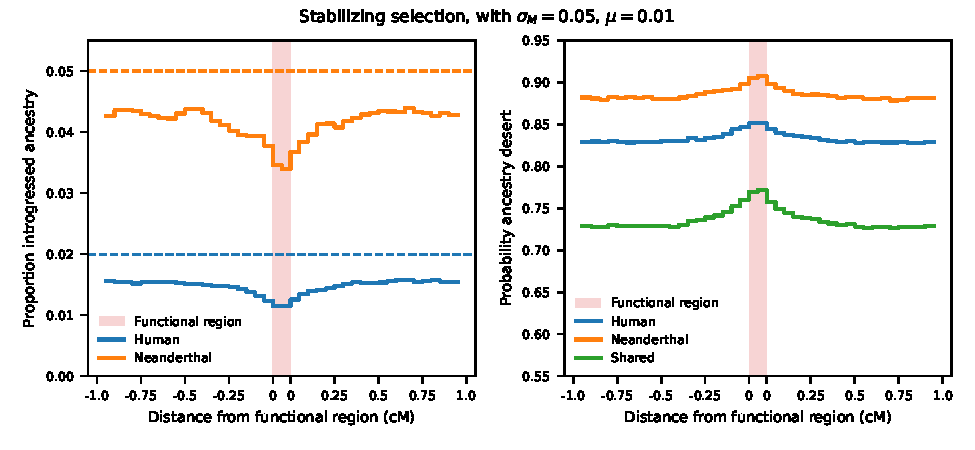
\includegraphics{../figures/introgression_deserts.SD_0.05.pdf}
    \caption{
        Introgressed ancestry and probability of introgression deserts in and
        around functional regions, from simulations with high mutational variance.
        The demographic model is shown in Figure~\ref{fig:human-neand-h2}A.
    }
    \label{fig:deserts-high-VM}
\end{figure}

\begin{figure}[ht!]
    \centering
    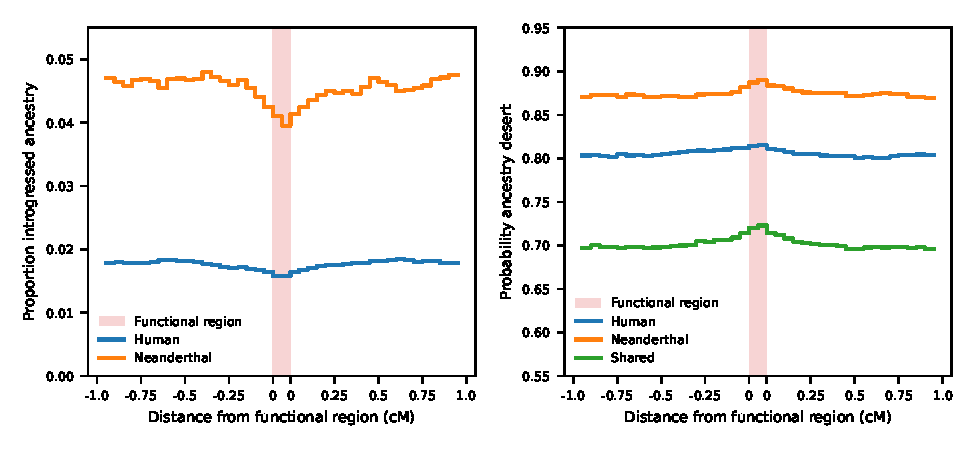
\includegraphics{../figures/introgression_deserts.SD_0.01.pdf}
    \caption{
        Introgressed ancestry and probability of introgression deserts in and
        around functional regions, from simulations with moderate mutational variance.
        The demographic model is shown in Figure~\ref{fig:human-neand-h2}A.
    }
    \label{fig:deserts-med-VM}
\end{figure}

\begin{figure}[ht!]
    \centering
    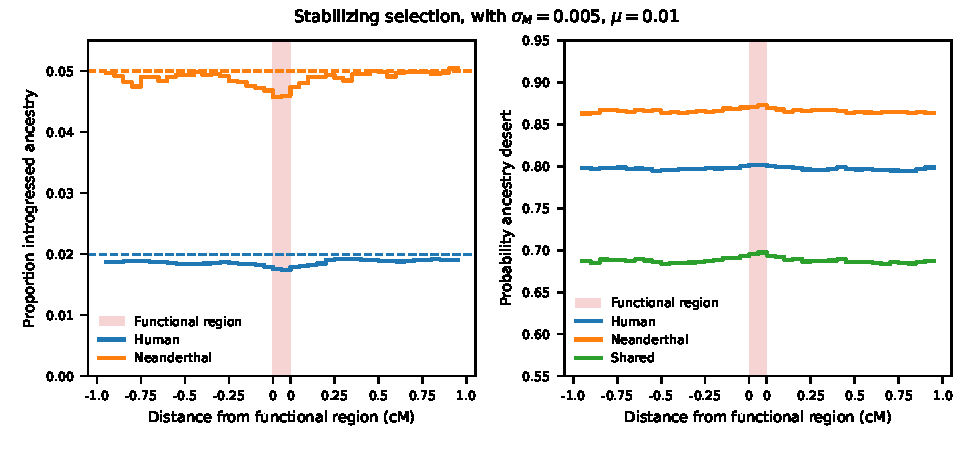
\includegraphics{../figures/introgression_deserts.SD_0.005.pdf}
    \caption{
        Introgressed ancestry and probability of introgression deserts in and
        around functional regions, from simulations with low mutational variance.
        The demographic model is shown in Figure~\ref{fig:human-neand-h2}A.
    }
    \label{fig:deserts-low-VM}
\end{figure}

\begin{figure}[ht!]
    \centering
    \includegraphics{../figures/introgression_deserts.directional.mean_-0.0002.shape_0.5.pdf}
    \caption{
        Introgressed ancestry and probability of introgression deserts in and
        around functional regions, from simulations with directional selection.
        Deleterious mutations were drawn from a gamma distribution with mean
        $-0.0002$ and shape $0.05$.
        The demographic model is shown in Figure~\ref{fig:human-neand-h2}A.
    }
    \label{fig:deserts-directional-A}
\end{figure}

\begin{figure}[ht!]
    \centering
    \includegraphics{../figures/introgression_deserts.directional.mean_-0.001.shape_0.5.pdf}
    \caption{
        Introgressed ancestry and probability of introgression deserts in and
        around functional regions, from simulations with directional selection.
        Deleterious mutations were drawn from a gamma distribution with mean
        $-0.001$ and shape $0.05$.
        The demographic model is shown in Figure~\ref{fig:human-neand-h2}A.
    }
    \label{fig:deserts-directional-B}
\end{figure}


\begin{figure}[ht!]
    \centering
    \includegraphics[width=0.6\textwidth]{../figures/underdominance_F2.pdf}
    \caption{
        Underdominance, like negative selection, reduces expected $F_2$ compared
        to neutral divergence.
    }
    \label{fig:underdominance-F2}
\end{figure}

\begin{figure}[ht!]
    \centering
    \includegraphics{../figures/supp-LD.pdf}
    \caption{
        Linkage disequilibrium between the a trait-affecting and neutral allele, 
        2000 generations after admixture. Inititally, the introgression proportion
        was $0.05$. Mutations with stronger effect sizes, and thus stronger selection
        against them, decrease in frequency more rapidly, leading to reduced LD
        as measured by $D=Cov(p,q)$ (Figure~\ref{fig:linkage}).
    }
    \label{fig:supp-LD}
\end{figure}

\begin{figure}[ht!]
    \centering
    \includegraphics[width=0.6\textwidth]{../figures/underdominance.Ne_10000.s_-5e-05.pdf}
    \caption{
        Comparison of predicted (\moments) and simulated SFS with underdominant
        selection. In this comparison, $N_e=10^4$ and $s=-5\times10^{-5}$, so that
        the population-size scale selection coefficient $\gamma=-1$.
        Simulations were performed under a Wright-Fisher model without linkage.
    }
    \label{fig:underdominance-validation-small-s}
\end{figure}

\begin{figure}[ht!]
    \centering
    \includegraphics[width=0.6\textwidth]{../figures/underdominance.Ne_5000.s_-0.001.pdf}
    \caption{
        Comparison of predicted (\moments) and simulated SFS with underdominant
        selection. In this comparison, $N_e=5000$ and $s=-0.001$, so that
        the population-size scale selection coefficient $\gamma=-10$.
        Simulations were performed under a Wright-Fisher model without linkage.
    }
    \label{fig:underdominance-validation-large-s}
\end{figure}

\begin{figure}[ht!]
    \centering
    \includegraphics[width=0.6\textwidth]{../figures/underdominance.Ne_5000.s_0.0005.pdf}
    \caption{
        Comparison of predicted (\moments) and simulated SFS with \emph{over}dominant
        selection. In this comparison, $N_e=5000$ and $s=0.0005$, so that
        the population-size scale selection coefficient $\gamma=5$.
        Thus, with positive selection, heterozygotes are favored.
        Simulations were performed under a Wright-Fisher model without linkage.
    }
    \label{fig:overdominance-validation}
\end{figure}


\end{document}
